\documentclass{beamer}
\usetheme{CambridgeUS}
\usecolortheme{rose}
\usepackage{braket}
\usepackage{tikz}
\usetikzlibrary{shapes,arrows}

\title{Computing P‐T Diagrams from First Principles}
%\author[me]{Max Tyler}
%\author[supervisor]{Miguel Martinez-Canales}
%\author{Max\inst{1}\\[1ex]  {\small supervisor1\inst{1,2}}
\author[Max Tyler]{Max Tyler\\{\small Supervisor: Dr. Miguel Martinez-Canales}}
\institute{The University of Edinburgh}
\date{April 2018}
 
 
 
\begin{document}
{ 
\usebackgroundtemplate
{
	\includegraphics[width=\paperwidth,height=\paperheight]{na9rlarge.png}
}
\frame{\titlepage}
}
 
\begin{frame}
	\frametitle{PT Diagrams}
	Pressure Temperature (PT) diagrams tell us what forms a structure exists in as a function of pressure and temperature.
	\pause
	\newline
	\newline
	Pressure and temperature most easily controllable variables in experiment.
	\pause
	\newline
	\newline
	How do we make them?
\end{frame}

\begin{frame}
	\frametitle{Density Functional Theory}
	Aim: Find the electron density, $n(\mathbf r)$ of some system.
	\begin{block}{Constrained Search for the Energy}<2->
		$$E_{v}[n] = \min_{\Psi \rightarrow n} \braket{\Psi|\hat T+\hat U + \hat V|\Psi} = F[n] + \int d^3\mathbf r n(\mathbf r) v_{ext}(\mathbf r)$$
	\end{block}
	\begin{block}{Kohn-Sham Formulation}<3->
		$$\left(-\frac{\hbar^2}{2m}\nabla^2+v_s(\mathbf r)\right)\phi_i(\mathbf r) = \epsilon_i \phi_i(\mathbf r),$$
		$$v_s(\mathbf r) = v_{ext}(\mathbf r) + v_H(\mathbf r) + v_{xc}(\mathbf r)$$
		$$n(\mathbf r) = \sum_i^N\phi^*_i(\mathbf r)\phi_i(\mathbf r)$$	
	\end{block}
\end{frame}

\begin{frame}
	\frametitle{Calculating the Electron Density}
	\tikzstyle{decision} = [diamond, draw, fill=blue!20, 
    text width=4.5em, text badly centered, node distance=3cm, inner sep=0pt]
\tikzstyle{block} = [rectangle, draw, fill=blue!20, 
    text width=6em, text centered, rounded corners, minimum height=4em]
\tikzstyle{line} = [draw, -latex']
\tikzstyle{cloud} = [draw, ellipse,fill=red!20, node distance=3cm,
    minimum height=2em]
    
\begin{tikzpicture}[node distance = 3.1cm, auto]
    % Place nodes
    \uncover<1->{\node [block] (init) {initial guess at charge density $n(\mathbf r)$};}
    \uncover<2->{\node [block, right of=init] (potential) {calculate new $v_s(\mathbf r)$ from $n(\mathbf r)$};}
    \uncover<3->{\node [block, right of=potential] (update) {solve Kohn-Sham equations for new $n(\mathbf r)=\sum_i \phi^*_i\phi_i$};}
    \uncover<4->{\node [decision, below of=update, node distance = 3.5cm] (decide) {are convergence criteria met?};}
    \uncover<5->{\node [block, right of=decide, node distance = 3.5cm] (stop) {output converged charge density};}
    % Draw edges
    \uncover<2->{\path [line] (init) -- (potential);}
    \uncover<3->{\path [line] (potential) -- (update);}
    \uncover<4->{\path [line] (update) -- (decide);}
    \uncover<5->{\path [line] (decide) -- node {yes} (stop);}
    \uncover<5->{\path [line] (decide) -| node {no}(potential);}
\end{tikzpicture}

\end{frame}
\begin{frame}
	\frametitle{Calculating Phonons}
	Need to use density functional perturbation theory.
\end{frame}

\begin{frame}
\frametitle{Silicon}
	\begin{figure}[ht]
	\begin{center}
	\includegraphics[height=2in]{sidiamond.png}
	\end{center}
	\end{figure}
\begin{center}
Silicon cell in diamond form
\end{center}
\end{frame}
 
\begin{frame}
	\frametitle{Silicon}
	\begin{figure}[ht]
	\begin{center}
	\includegraphics[height=2in]{silicon_0_500_comparison.png}
	\end{center}
	\end{figure}
\end{frame}

\begin{frame}
	\frametitle{Silicon}
	\begin{columns}
\column{0.5\textwidth}
	\begin{figure}[ht]
	\begin{center}
	\includegraphics[height=1.8in]{silicon_isotherms.png}
	\end{center}
	\end{figure}
\column{0.5\textwidth}
	\begin{figure}[ht]
	\begin{center}
	\includegraphics[height=1.8in]{silicon_min_volume.png}
	\end{center}
	\end{figure}
\end{columns}
\end{frame}

\begin{frame}
	\frametitle{Silicon's Coefficient of Linear Thermal Expansion}
	\begin{figure}[ht]
	\begin{center}
		\includegraphics[height=2in]{silicon_thermal_expansion.png}
	\end{center}
	\end{figure}
\end{frame}

\begin{frame}
\frametitle{Tin}
\begin{center}Calculating the transition temperature between $\alpha$ and $\beta$ tin\end{center}
\begin{columns}
\column{0.4\textwidth}
	\begin{figure}[ht]
	\begin{center}
		\includegraphics[height=1.3in]{alphasn.png}
	\end{center}
	\end{figure}
	\begin{center}
		$\alpha$-Tin
	\end{center}
\column{0.4\textwidth}
	\begin{figure}[ht]
	\begin{center}
		\includegraphics[height=1.3in]{betasn.png}
	\end{center}
	\end{figure}
	\begin{center}
		$\beta$-Tin
	\end{center}
\end{columns}
\end{frame}

\begin{frame}
	\frametitle{Tin Phase Transition}
	\begin{figure}[ht]
	\begin{center}
	\includegraphics[height=2in]{tin_transition_temperature.png}
	\end{center}
	\end{figure}
\pause
\begin{center}Much larger transition temperature than is observed experimentally $(\approx 290K)$. Problem with PBE functional, which can be fixed with $+U$ correction. \footnote{F. Legrain et. al. AIP Advances 6, 045116 (2016)}\end{center}
\end{frame}

\begin{frame}
	\frametitle{Sodium Crystal Structure}
	\begin{columns}
\column{0.3\textwidth}
	\begin{figure}[ht]
	\begin{center}
		\includegraphics[height=1.3in]{nabcccrystal.png}
	\end{center}
	\end{figure}
	\begin{center}
		BCC
	\end{center}
\column{0.3\textwidth}
	\begin{figure}[ht]
	\begin{center}
		\includegraphics[height=1.3in]{nafcccrystal.png}
	\end{center}
	\end{figure}
	\begin{center}
		FCC
	\end{center}
\column{0.3\textwidth}
	\begin{figure}[ht]
	\begin{center}
		\includegraphics[height=1.23in]{na9rcrystal.png}
	\end{center}
	\end{figure}
	\begin{center}
		9R
	\end{center}
\end{columns}
\end{frame}
\begin{frame}
	\frametitle{Sodium PT Diagram}
	\begin{figure}[ht]
	\begin{center}
		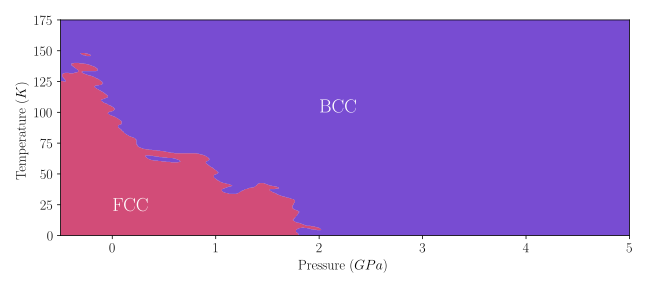
\includegraphics[height=2in]{sodium_pt_diagram.png}
	\end{center}
	\end{figure}
\end{frame}

\begin{frame}
	\frametitle{}
\end{frame}

\begin{frame}
	\frametitle{Further Research}
	Look into other phases in this region (HCP, etc.)
\end{frame}

\end{document}

